% Preamble
\documentclass [11pt]{article}

\usepackage{setspace}
\usepackage{amssymb}
\usepackage{amsmath}
\usepackage{amsfonts}
\usepackage{amssymb}
\usepackage{setspace}
\usepackage{amsthm}
\usepackage{textcomp}
\usepackage{graphicx}
\usepackage{url}
\usepackage{color}
\usepackage[dvipsnames]{xcolor}
\definecolor{cuteBlue}{rgb}{0.258, 0.387, 0.574}
\definecolor{cuteGreen}{rgb}{0, 0.3, 0}
\usepackage{cancel}
\usepackage{comment}
\usepackage[framemethod=TikZ]{mdframed}
\usepackage{enumitem}
\usepackage{wasysym}
\usepackage{listings}
\usepackage{float}
\usepackage{booktabs}
\usepackage{fixltx2e}
\usepackage{threeparttable}
\usepackage{titling}
\usepackage{zref-base}
\usepackage{makecell}
\usepackage{array}
\usepackage{hhline}
\usepackage{titlesec}
\usepackage{tcolorbox}

% To make jumping between equation, figure, citation references easier
\usepackage[colorlinks=true, urlcolor=cuteBlue, citecolor=cuteGreen, linkcolor=black]{hyperref}

% To make caption labels (i.e. Figure 1, Figure 2...) bold and
% make all caption text small
\usepackage[labelfont=bf, font=small]{caption}

% For strike-out text during editing
\usepackage[normalem]{ulem}

%Latin accents
\usepackage[utf8]{inputenc}

%subfigures
\usepackage{caption}

% Add author affiliations
\usepackage{authblk}

% %%%%%%%%%%%%%%%%%%%%%%%%%%%%%%%%%%%%%%%%%%%%%%%%%%%%%%%%%%%%%%%%%%%%%%%%%%%%%%
% %%%%%%%%%%%%%%%%%%%%%%%%%%%%%%%%%%%%%%%%%%%%%%%%%%%%%%%%%%%%%%%%%%%%%%%%%%%%%%

% Margins and spacings
\setlength{\evensidemargin}{0.0cm}
\setlength{\oddsidemargin}{0.0cm}
\setlength{\topmargin}{-1.0cm}
\setlength{\textwidth}{17cm}
\setlength{\textheight}{22cm}
\setlength{\parskip}{2.5mm}
\reversemarginpar
\marginparsep  0.1in
\marginparwidth 0.7in

% Give more spacing in equation arrays
\setlength{\jot}{10pt}

% Allow page breaks in multiline equations
\allowdisplaybreaks

% Set up title spacing so we don't waste so much space
\setlength{\droptitle}{-8em}
\date{\vspace{-5em}}  % No date will appear in title.

% Spacing between section headings and text
\titlespacing\section{0pt}{12pt plus 4pt minus 2pt}{-2pt plus 2pt minus 2pt}
\titlespacing\subsection{0pt}{12pt plus 4pt minus 2pt}{-2pt plus 2pt minus 2pt}
\titlespacing\subsubsection{0pt}{12pt plus 4pt minus 2pt}{-2pt plus 2pt minus 2pt}

% Convenient micron symbol
\newcommand{\micron}{{\textmu}m}

% No excess spacing for lists
\setlist{itemsep=0pt, topsep=0pt}

% Allow paragraph indentations in lists
\setitemize{listparindent=\parindent}
\setenumerate{listparindent=\parindent}

% Column type for tables with nice spacing
\newcolumntype{M}[1]{>{\centering\arraybackslash}m{#1}}
\newcolumntype{N}{@{}m{0pt}@{}}


% %%%%%%%%%%%%%%%%%%%%%%%%%%%%%%%%%%%%%%%%%%%%%%%%%%
% Document settings
% %%%%%%%%%%%%%%%%%%%%%%%%%%%%%%%%%%%%%%%%%%%%%%%%%%

% References
\usepackage[
	backend=bibtex,
	style=numeric-comp, % show references as [1-3] instead of [1,2,3]
	sorting=none,				% Do not sort bibliography
	url=false, 					% Do not show url in reference
	doi=false, 					% Do not show doi in reference
	isbn=false, 				% Do not show isbn link in reference
	eprint=false, 			% Do not show eprint link in reference
	maxbibnames=9, 			% Include up to 9 names in citation
]{biblatex}
% Add library
\addbibresource{./chann_cap_bib}

% Bold the 'Figure #' in the caption and separate it from the title/caption
% with a period
% Captions will be left justified
\usepackage[
	aboveskip=1pt,
	labelfont=bf,
	labelsep=period,
	justification=raggedright,
	singlelinecheck=off
]{caption}

% Add numbered lines
\usepackage{lineno}
\linenumbers

% Package to include multiple title pages
% This will allow me to add a tile to the main text and to the SI
\usepackage{titling}

% This package will allow me to define booleans to compile main text or SI
\usepackage{ifthen}
\newboolean{maintext}
\newboolean{sitext}

%%%%%%%%%%%%%%%%%%%%%%%%%%%%%%%%%%%%%%%%%%%%%%%%%%%%
% Personalized functions
%%%%%%%%%%%%%%%%%%%%%%%%%%%%%%%%%%%%%%%%%%%%%%%%%%%%
% Commenting
\newcommand{\mrm}[1]{\textcolor{cuteBlue}{(MR:~#1)}} % Commenting
\newcommand{\rp}[1]{\textcolor{red}{(RP:~#1)}} % Commenting
\newcommand{\note}[1]{\textcolor{ForestGreen}{(NOTE~#1)}} % Commenting

% To define more useful LaTeX commands
\usepackage{xparse}

% Equation referencing
\newcommand{\eref}[1]{Eq.~\ref{#1}}
% Figure referencing
\newcommand{\fref}[1]{Fig.~\ref{#1}}
% Table referencing
\newcommand{\tref}[1]{Table~\ref{#1}}
% Section referencing
\newcommand{\secref}[1]{Section~\ref{#1}}
% SI referencing
\newcommand{\siref}[1]{Appendix~\ref{#1}}

% Define command to begin the supplementary section
\newcommand{\beginsupplement}{
				\setcounter{section}{0} % Restart section counter
        \renewcommand{\thesection}{S\arabic{section}}%
        \setcounter{table}{0} % Restart table counter
        \renewcommand{\thetable}{S\arabic{table}}%
        \setcounter{figure}{0} % Restart figure counter
        \renewcommand{\thefigure}{S\arabic{figure}}%
        \setcounter{equation}{0} % Restart equation counter
        \renewcommand{\theequation}{S\arabic{equation}}%
     }

%%%%%%%%%%%%%%%%%%%%%%%%%%%%%%%%%%%%%%%%%%%%%%%%%%%%
% Personalized math functions
%%%%%%%%%%%%%%%%%%%%%%%%%%%%%%%%%%%%%%%%%%%%%%%%%%%%
% Vector P (for distribution vector)
\newcommand{\PP}{\bb{P}}
% Expected value
\newcommand{\ee}[1]{\left\langle #1 \right\rangle}
% Bold math
\newcommand{\bb}[1]{\mathbf{#1}}
% Time derivative
\newcommand{\dt}[1]{{d{#1} \over dt}}
\newcommand{\ddt}[1]{{\partial{#1} \over \partial t}}

%%%%%%%%%%%%%%%%%%%%%%%%%%%%%%%%%%%%%%%%%%%%%%%%%%%%
%% Begin document
%%%%%%%%%%%%%%%%%%%%%%%%%%%%%%%%%%%%%%%%%%%%%%%%%%%%

\title{
\textbf{Statistical Gentics Notes}
}
% Authors
\author[1]{Manuel Razo-Mejia}
\author[1, 2, 3, *]{Rob Phillips}

% Affiliations
\affil[1]{Division of Biology and Biological Engineering, California Institute
of Technology, Pasadena, CA 91125, USA}
\affil[2]{Department of Physics, California Institute of Technology, Pasadena,
CA 91125, USA}
\affil[3]{Department of Applied Physics, California Institute of Technology,
Pasadena, CA 91125, USA}
\affil[*]{Correspondence: phillips@pboc.caltech.edu}

% date
% \date{\today}

\setcounter{Maxaffil}{0}
% Set affiliations in small font
\renewcommand\Affilfont{\itshape\small}

\begin{document}
%% MAIN TEXT
\maketitle % Set title for paper

% Chapter 1. Probability theory
% !TEX root = ../../main.tex
\section{Classic diffusion theory in population genetics}

The pioneers of the modern-synthesis of evolution established solid foundations
for how to understand the different forces at play that shape the structure of
evolving populations. But combining all of these forces into a single
description remained challenging. In other words, describing the outcome of an
evolutionary process that combined deterministic processes such as selection
and mutation with the stochasticity of evolution presented a challenging
mathematical puzzle. The first attempt to put everything together came from
Sewall Wright himself, but the achievement of formalizing the theory is often
associated with a remarkable Japanese population genetics by the name of Motoo
Kimura.

Kimura jump to fame when in 1968 he presented his \textit{Neutral theory of
molecular evolution}. In here Kimura argued that associating every biological
aspect to the outcome of a selection-driven process was too much of a naive
picture. We previously mentioned that Wright thought about genetic drift as an
important component of the evolutionary process, but in this 1968 paper Kimura
argued that it was \textit{the} dominant force in evolution.

But what really brings us here to study part of Kimura's scientific legacy is
his use of diffusion equations in the context of population genetics. What we
know now as Kimura's diffusion theory is nothing else than the application of
the mathematical tools developed for the study of physical diffusion of
particles to evolving populations. Diffusion is one of several transcendent
concepts in physics that demonstrate the power of universal concepts. The same
equation that describes how the concentration of a chemical species changes as
a function of space and time is used to describe how the temperature profile of
an object changes as a function of space and time as well. Furthermore, as we
will study in this section, the same mathematical language can describe
diffusion on an abstract space of allele frequency. So as Joe Blitzstein likes
to say: ``nouns change, but the verbs remain the same.''

The mathematical language to study diffusion theory, as with many other field
of science is the language of probability theory. As Jaynes' famous book title
suggested, \textit{probability theory is the logic of science}. It is through
this formal language that we can assess how likely are specific events to
happen. For example, later on we'll see that within the framework of diffusion
theory is possible to ask what is the probability of an allele being fixed in
the population given the evolutionary forces acting on it. In particular we are
interested in a type of probability object known as a Markov process that we
will now define.

\subsection{Markov processes}
Of particular interested for our endeavor are the specific mathematical objects
known as Markov processes. The Markovian property - named after Andrey Markov,
a famous Russian mathematician from the XIX century - can be stated as follows:
A Markov process is a type of stochastic process for which the transition
states only depends on the current state.

To gain intuition for what this means imagine we are measuring a variable $x$
over time such that we have a bunch of pairs of the form $(x_1, t_1), (x_2,
t_2), (x_3, t_3), \ldots (x_{n+1}, t_{n+1})$. For a Markov process, the
probability of ending at state $x_{n+1}$ at time $t_{n+1}$ given all the
previous visited states is of the form
\begin{equation}
  P(x_{n+1}, t_{n+1} \mid x_1, t_1; x_2, t_2; \ldots; x_n, t_n) =
  P(x_{n+1}, t_{n+1} \mid x_n, t_n).
  \label{eq_chapman_kolmogorov}
\end{equation}
In other words, knowing the entire history of variable $x$ as it evolves over
time does not help us predict the next time step. All we need to know is the
last position. Markov processes are usually called memoryless stochastic
process because of this property that the process doesn't remember the full
trajectory when it ``decides'' where to move in the next step. Assuming a
Markovian process is arguably one of the most widely used assumptions in all of
science; from chemical reactions, to brownian motion of a particle, to our
particular case of interest of allele frequencies changing over time.

In the classic formulation of diffusion theory we are concerned with a
particular type of Markov processes. Diffusion theory works in the limit of
large populations where we can assume that the frequency of a particular allele
rather than being a discrete entity that changes in factors of $1 / N$ where
$N$ is the number of organisms, is a continuous value in the range between 0
and 1. We also assume that we can compute changes in this frequency in
continuous time. That means that both $f$ the frequency of an allele, and $t$
the time are continuous variables. Therefore we are interested in a type of
Markov processes that go by the creative name of continuous-time
continuous-state Markov processes. We will now state a very important equation
for this type of Markovian processes known as the Chapman-Kolmogorov equation.

\subsubsection{Chapman-Kolmogorov equation} \label{sec_chapman_kolmogorov}

The Chapman-Kolmogorov equation is an important property of continuous-time
continuous-state Markov processes that we will use for many of our derivations
in the coming sections. The equation is stated as follows: For three time points
$t_1 < t_2 < t_3$ for which we measured a stochastic variable $x$ we have that
\begin{equation}
  P(x_3, t_3 \mid x_1, t_1) = \int dx_2\; P(x_3, t_3 \mid x_2, t_2)
                                          P(x_2, t_2 \mid x_1, t_1),
\end{equation}
where the integral is taken over the domain of values that the random variable
$x$ can take. In other words, to calculate the transition probability between
$x_1$ and $x_3$ with an intermediary step $x_2$, we must add (integrate for
continuous variables) all possible values that $x_2$ can take. This concept is
schematically represented in \fref{fig_03_02_01}

\begin{figure}[h!]
	\centering 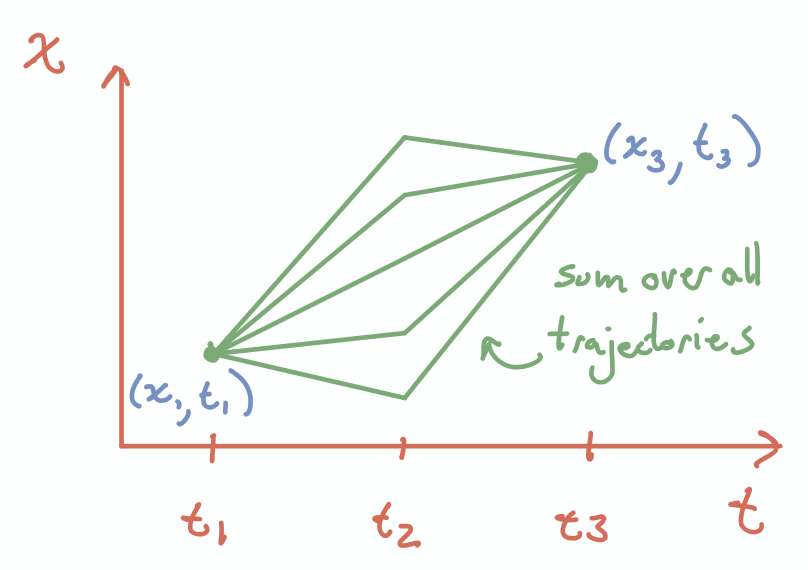
\includegraphics[width=0.5\textwidth]
  {../fig/classic_diffusion/03_02_01_chapman_kolmogorov.png}
	\caption{\textbf{Schematic of the Chapman-Kolmogorov equation}. The
  Chapman-Kolmogorov equation is a statement about the transition between two
  points $x_1$ and $x_3$, adding all possible intermediary steps $x_2$.}
  \label{fig_03_02_01}
\end{figure}

In the coming section we will use the Chapman-Kolmogorov equation to derive the
so-called continuous master equation. This will be the foundation from which we
will get to the main results of diffusion theory. But before jumping into such
matter we need to introduce a specific subtype of Markov processes.

\subsubsection{Stationary Markov Process}\label{sec_stationary_process}

When thinking about evolution we often summon the concept of a mapping between
genotype (sequence level description) to phenotype (observable characteristic)
to fitness (reproductive success). This concept goes by several names, but in
1932 Sewall Wright attempted to formalize this idea as \textit{adaptive
landscapes}. The phenotype itself can be a function of the genotype and the
environmental state that can itself change over time either deterministically
or stochastically. Therefore the idea of a ``landscape'' is not necessarily the
best description. Some authors have discussed concepts such as \textit{fitness
seascapes} when the environment evolves over time independently of the organism
or \textit{fitness snowscapes} when there is a direct interaction between
organisms modifying the environment, and the environment modifying the
organisms.

For simplicity we usually work with fixed fitness landscapes. This
approximation is valid under certain time-scale regimes. For example, if the
environment does change over time, but it does it on a time-scale much longer
than what it takes for organisms to adapt, then we can pretend for our
calculations that the environment is fixed, simplifying the math enormously.
For this particular case where the mapping all the way from genotype to fitness
is not a function of time is described by a type of stochastic chain known as
\textbf{stationary Markov process}. The formal definition of a stationary
Markov process can be stated as: A stationary Markov process is a memoryless
process for which when computing the moments of the distribution, these are not
affected by a time shift $\tau$, i.e.
\begin{equation}
  \ee{X(t_1 + \tau) X(t_2 + \tau) \cdots X(t_n + \tau)} =
  \ee{X(t_1) X(t_2) \cdots X(t_n)}.
\end{equation}
In other words, for a stationary Markov process what matters are the absolute
time differences $|t_2 - t_1|$ rather than the absolute time points. This
implies that the probability of our random variable having a particular value
$x$ is governed by a probability distribution $P_X(x)$ with no time dependence.
Notice the difference between the statements: On the one hand if we want to
know what is the probability of the random variable transitioning from a value
$x$ to a value $x'$ all we need to know is how much time passed between both
instances of the random process. On the other hand if we are only interested in
knowing what is the probability of the random variable taking a specific value
there is no time dependence for a stationary process since this probability
will not change over time. For the evolution questions we will be addressing
here is easy to see how this implies a fixed adaptive landscape. Since the
environment is fixed the mapping between genotype all the way to fitness will
be the same regardless of the time at which the population acquires a specific
allele frequency.

Now we are ready to derive the master equation that will describe the time
evolution of the probability distribution of allele frequencies.
\section{The (continuous) master equation for allele frequencies}

One of the most powerful tools to study stochastic process is the so-called
master equation. Originally devised to study the stochastic time evolution of
chemical reactions - thereby christened the chemical master equation - this
equation has found applications in many areas of chemistry, physics and biology.
The equation is as statement about the time evolution of the transition
probabilities of a Markov process. That is just a fancy way of saying that the
master equation describes how the transition probabilities between states change
over time.

Let's derive this powerful equation starting from \eref{eq_chapman_kolmogorov}.
For our case of study we want to understand how the frequency of a particular
allele evolves over time, that is a stochastic process $F(t)$. Notice again that
we distinguish between the stochastic process $F(t)$ formed by the ensemble of
all possible realizations $f(t)$. The Chapman-Kolmogorov equation for this
particular case with three time points $t_1 < t_2 < t_3$ takes the form
\begin{equation}
  P(f_3, t_3 \mid f_1, t_1) = \int_0^1 df_2\; P(f_3, t_3 \mid f_2, t_2)
                                          P(f_2, t_2 \mid f_1, t_1),
  \label{eq_chapman_freq}
\end{equation}
where the integration limits $[0, 1]$ are the domain of values that an allele
frequency can take. Now let us assume that we observe the frequency at time $t$
and it happens to be at a value $f_1$. Then after a very short time $\Dt$ we
observe again the allele frequency which is now at a value $f_2$. Under this
short time limit we can approximate the transition probability as
\begin{equation}
  P(f_2, t + \Dt \mid f_1, t) = \delta(f_2 - f_1)
  \underbrace{\left[ 1 - a^{(0)}(f_1, t) \Dt \right]}_{\text{probability
  of no transition}} +
  \underbrace{\phi_t(f_2 \mid f_1)\Dt}_\text{probability of transition} +
  \mathcal{O}(\Dt^2).
  \label{eq_transition_short_time}
\end{equation}
Let's break down this equation. We have split the possible things that can
happen on a time window $\Dt$ into two possible cases. The first one represented
by the first term on the right-hand side is the possibility that on this small
time window no transition actually takes place. The $\delta$-function that is
equal to 1 if and only if $f_2 = f_1$ is there to make sure that this term is
added only when there was no transition during that time and $f_2$ remains the
same as $f_1$. Inside the square brackets we wrote $1 - a^{(0)}(f_1, t) \Dt$,
the reason for writing the term $a^{(0)}$ will become clear later on when we
derive the so-called Fokker-Planck equation. Having a term of the form 1 -
``something'' hints at the fact that this ``something'' must be the probability
of transitioning somewhere else rather than staying at the same position. For
the second term we wrote $\phi_t(f_2 \mid f_1)\Dt$ as the probability of
transitioning outside of $f_1$ during this time window. our function $\phi_t(f_2
\mid f_1)$ represents the transition probability per unit time between $f_1$ and
$f_2$ at time $t$. When we multiply this rate in time$^{-1}$ units by a small
time window, we obtain the probability of transitioning from $f_1$ to $f_2$.

In order to understand better the term $a^{(0)}(f_1, t)$ in
\eref{eq_transition_short_time} recall that a probability distribution must be
normalized. That means that if we integrate both sides of
\eref{eq_transition_short_time} over all values of $f_2$ it must be true that
\begin{equation}
  \int_0^1 df_2 \; P(f_2, t + \Dt \mid f_1, t) =
  \int_0^1 df_2 \; \delta(f_2 - f_1) \left[ 1 - a^{(0)}(f_1, t) \Dt \right]
  + \int_0^1 df_2 \; \phi_t(f_2 \mid f_1)\Dt
  = 1.
\end{equation}
Integrating over the $\delta$-function implies that we set $f_2 = f_1$,
therefore we obtain
\begin{equation}
  1 = \left[  1 - a^{(0)}(f_1, t) \Dt\right] +
  \int_0^1 df_2 \; \phi_t(f_2 \mid f_1)\Dt.
\end{equation}
Solving for $a^{(0)}(f_1, t)$ results in
\begin{equation}
  a^{(0)}(f_1, t) = \int_0^1 df_2 \; \phi_t(f_2 \mid f_1),
  \label{eq_a0}
\end{equation}
proving our previous assertion that $a^{(0)}(f_1, t)$ must be the
probability of jumping from $f_1$ to somewhere else.

Using this approximation for short time steps we will now derive the
differential equation that the transition probability between frequencies must
obey. Specifically for three time points $t_o < t < t + \Dt$ with corresponding
allele frequencies $f_o, f', f$ we have that \eref{eq_chapman_freq} takes the
form
\begin{equation}
  P(f, t + \Dt \mid f_o, t_o) = \int_0^1 df' \; P(f, t + \Dt \mid f', t)
  P(f', t \mid f_o, t_o).
\end{equation}
Substituting \eref{eq_transition_short_time} results in
\begin{equation}
  P(f, t + \Dt \mid f_o, t_o) = \int_0^1 df' \;
  \left[ \delta(f - f') \left( 1 - a^{(0)}(f', t)\Dt \right)
  + \phi_t(f \mid f')\Dt \right]
  P(f', t \mid f_o, t_o).
\end{equation}
Evaluating the integral for the first term on the right-hand side gives
\begin{equation}
  P(f, t + \Dt \mid f_o, t_o) = \left[\left( 1 - a^{(0)}(f, t)\Dt \right)\right]
  P(f, t \mid f_o, t_o) +
  \Dt \int_0^1 df' \; \phi_t(f \mid f') P(f', t \mid f_o, t_o).
\end{equation}
We can then substitute \eref{eq_a0} and rearrange terms to obtain
\begin{equation}
  P(f, t + \Dt \mid f_o, t_o) = P(f, t \mid f_o, t_o)
  + \int_0^1 df' \left[ \phi_t(f \mid f') P(f', t \mid f_o, t_o) -
  \phi_t(f' \mid f) P(f, t \mid f_o, t_o) \right]\Dt.
\end{equation}
Sending the first term on the right-hand side to the left, dividing both sides
by $\Dt$ and taking the limit $\Dt \rightarrow 0$ gives the differential
equation we were looking for
\begin{equation}
  \dt{P(f, t \mid f_o, t_o)} = \int_0^1 df' \;
  \underbrace{
  \left[ \phi_t(f \mid f') P(f', t \mid f_o, t_o) \right.}
  _{\text{gain } f' \rightarrow f}  -
  \underbrace{
  \left. \phi_t(f' \mid f) P(f, t \mid f_o, t_o) \right]}
  _{\text{loss } f \rightarrow f'}.
  \label{eq_master_eq_trans}
\end{equation}
This is the integro-differential equation known as the master equation. This
continuous form of the master equation describes the time evolution of the
transition probabilities $P(f, t \mid f_o, t_o)$, not the evolution of the
probability of being at a specific state $P(f, t)$. However we can use the rules
of probability to obtain such description by the following process: Suppose the
stochastic process $F(t)$ describes the time evolution of the frequency.
Assuming $F(t)$ is a stationary Markov process as described in
\secref{sec_stationary_process} means that this process is completely
characterized by two functions - the probability of having a particular value
for the allele frequency $P_F(f)$ that does not depend on time, and a transition
probability $P(f, t \mid f_o, t_o)$. We define a new, non-stationary process
$F^*(t)$ for $t \geq t_o$ by setting
\begin{equation}
  P^*(f, t) = P(f, t\mid f_o, t_o),
\end{equation}
i.e. forcing the initial condition to be a specific value $f_o$ at time $t_o$.
This is a sub-ensemble of the process $F(t)$ since we demanded that $F(t = t_o)
= f_o$. More generally if instead of setting the initial condition to be a
single specific value $P(f, t_o) = \delta(f - f_o)$ we define a probability
distribution for the initial state $P(f, t_o) = \rho(f_o)$, we have a
sub-ensemble of the form
\begin{equation}
  P^*(f, t) = \int_0^1 df_o \; P(f, t\mid f_o, t_o) \rho(f_o).
  \label{eq_subensemble}
\end{equation}
The interpretation of this sub ensemble is that the system was initially set on
a non-stationary state. The initial state distribution $\rho(f_o)$ does not
depend on time, therefore if we take the time derivative on both sides of
\eref{eq_subensemble} we find that
\begin{equation}
  \dt{P^*(f, t)} = \int_0^1 df_o \; \dt{P(f, t\mid f_o, t_o)}
                        \rho(f_o).
\label{eq_subensemble_dt}
\end{equation}
Notice that the term with the time derivative on the right-hand side of
\eref{eq_subensemble_dt} is the master equation that we derived in
\eref{eq_master_eq_trans}. Substituting this results in
\begin{equation}
  \dt{P^*(f, t)} = \int_0^1 df_o \; \rho(f_o)
  \int_0^1 df' \;
  \left[ \phi_t(f \mid f') P(f', t \mid f_o, t_o) -
  \phi_t(f' \mid f) P(f, t \mid f_o, t_o) \right].
\end{equation}
Redistributing the integrals gives
\begin{equation}
  \dt{P^*(f, t)} = \int_0^1 df' \; \phi_t(f \mid f')
  \overbrace{
  \int_0^1 df_o \; P(f', t \mid f_o, t_o) \rho(f_o)}
  ^{P^*(f', t)\text{ by definition}} -
  \int_0^1 df' \; \phi_t(f' \mid f)
  \overbrace{
  \int_0^1 df_o \; P(f, t \mid f_o, t_o) \rho(f_o)}
  ^{P^*(f, t)\text{ by definition}}.
\end{equation}
Using the definition of the sub-ensembles shown in \eref{eq_subensemble} we
arrive to a result of the form
\begin{equation}
  \dt{P^*(f, t)} = \int_0^1 df' \;
  \underbrace{
  \phi_t(f \mid f') P^*(f', t)
  }_{f' \rightarrow f \text{ gain}} -
  \int_0^1 df' \;
  \underbrace{
  \phi_t(f' \mid f) P^*(f, t)
  }_{f \rightarrow f' \text{ loss}}.
  \label{eq_master_eq_full}
\end{equation}
In this form we can see that the master equation is a balance between gain and
loss of probability at each state $f$. Having said that, the truth about the
continuous master equation is that is extremely complicated to work with. In
general integro-differential equations are challenging mathematical objects to
deal with. That is why in the next section we'll use the powerful tool of
Taylor expansions to simplify the equation. But before that let's discuss some
historic uses of the master equation that might look different to our derivation
on \eref{eq_master_eq_full}.

\subsection{Einstein-Kimura continuous master equations}

In 1905 during the groundbreaking year of Einstein's scientific career he
published a paper in which he attempted to give a molecular explanation to the
phenomena of Brownian motion. For this he derived Fick's second law from of a
statistical argument by Taylor expanding a master equation - more on that in
the next section. In this classic paper Einstein had one of the very first uses
of a continuous master equation applied to a physical problem. The difference
from our approach is that Einstein didn't derive the master equation from the
Chapman-Kolmogorov property of continuous-time continuous-state Markov
processes, but simply proposed its functional form directly.

While the problem Einstein was addressing in his paper had to do with a random
walker moving in real space, the mathematical tools that he proposed can be
directly mapped to the population genetics setup. As a matter of fact Motoo
Kimura himself used an equivalent approach to Einstein's formulation of the
master equation for his formulation of diffusion theory. Kimura used the same
approach as Einstein of Taylor expanding the master equation, with the main
difference being that for population genetics the transition probability
$\phi_t(f \mid f')$ is a function of the current position $f'$ while in real
space free diffusion is independent of the position. For this short section our
objective is to show that our derivation of the master equation is equivalent to
Einstein's and Kimura's proposed functional form. We will focus on Kimura's
version of the master equation since population genetics is what concerns us in
these notes.

Kimura's original derivation of the classic diffusion theory begins stating that
the process of allele frequency changes can be stated as
\begin{equation}
  P(f, t + \Dt) = \int d\varepsilon \;
  P(f - \varepsilon, t) \phi_t(f \mid f - \varepsilon) \Dt,
  \label{eq_kimura_master}
\end{equation}
and that is it. While it took us a while to justify \eref{eq_master_eq_full},
Kimura (and Einstein in the context of Brownian motion) simply stated the master
equation as the starting point. There is nothing intrinsically wrong about
having \eref{eq_kimura_master} as the starting point, but in this set of extend
notes I thought it would be insightful to start from a more fundamental property
of Markov processes and have the master equation be a consequence of such
property. Also I would like to highlight that in all of the population genetics
literature I have come across so far there has never been an explicit account of
the integration limits on the equations. This includes Kimura's original work as
well as textbooks. For this particular case the integration limits should go
from $f$ to $f - 1$ such that the values of $f - \varepsilon$ range from 0 to 1.
So the proper form of this integral is given by
\begin{equation}
  P(f, t + \Dt) = \int_{-f}^{f - 1} d\varepsilon \;
  P(f - \varepsilon, t) \phi_t(f \mid f - \varepsilon) \Dt.
  \label{eq_kimura_master_lim}
\end{equation}

Notice that at first glance \eref{eq_master_eq_full} and
\eref{eq_kimura_master_lim} don't seem to be equivalent.
\eref{eq_master_eq_full} is a differential equation that describes how the
probability distribution changes given gains and losses of probability on state
$f$, while \eref{eq_kimura_master_lim} only makes a statement of what would the
probability distribution look like a tiny time step into the future by adding
all the jumps \textbf{into} state $f$, but it doesn't include a term for all the
jumps out of state $f$. To show that these equations are equivalent we have to
do two things:
\begin{enumerate}
  \item On \eref{eq_master_eq_full} we notice that the second term on the
  right-hand side can be written as
  \begin{equation}
    P^*(f, t)\int_0^1 df' \; \phi_t(f' \mid f) = P^*(f, t),
    \label{eq_integral_transition}
  \end{equation}
  where we took the term $P^*(f, t)$ outside of the integral and used the fact
  that the transition probability per unit time $\phi_t(f' \mid f)$ should be
  normalized regardless of the time window. In other words, the probability of
  transitioning from $f$ to anywhere else (including staying at $f$) should add
  up to one regardless of the time window we observe.
  \mrm{Need to check this statement and that the units make sense}
  \item Having this result we can rewrite \eref{eq_master_eq_full} as
  \begin{equation}
    \dt{P^*(f, t)} = \int_0^1 df' \;
    \phi_t(f \mid f') P^*(f', t) - P^*(f, t).
    \label{eq_master_eq_rearange}
  \end{equation}
  We are almost there! All is left is to notice that if we were to Taylor expand
  the left-hand side of \eref{eq_kimura_master_lim} with respect to time up to
  first order (as it is often done for time derivatives) we would obtain
  \begin{equation}
    P(f, t + \Dt) = P(f, t) + \dt{P(f, t)}\Dt + \mathcal{O}(\Dt^2).
  \end{equation}
  That means we can send the second term on the the right-hand side of
  \eref{eq_master_eq_rearange} to the left and rewrite the equation as
  \begin{equation}
    {P^*(f, t + \Dt) \over \Dt} = \int_0^1 df' \;
    \phi_t(f \mid f') P^*(f', t),
  \end{equation}
  which is equivalent to \eref{eq_kimura_master_lim} where instead of having
  the integration over the jump size $\varepsilon$ the integration is done over
  the final position $f'$.
\end{enumerate}


\end{document}
